% Options for packages loaded elsewhere
\PassOptionsToPackage{unicode}{hyperref}
\PassOptionsToPackage{hyphens}{url}
\PassOptionsToPackage{dvipsnames,svgnames,x11names}{xcolor}
%
\documentclass[
  letterpaper,
  DIV=11,
  numbers=noendperiod]{scrartcl}

\usepackage{amsmath,amssymb}
\usepackage{iftex}
\ifPDFTeX
  \usepackage[T1]{fontenc}
  \usepackage[utf8]{inputenc}
  \usepackage{textcomp} % provide euro and other symbols
\else % if luatex or xetex
  \usepackage{unicode-math}
  \defaultfontfeatures{Scale=MatchLowercase}
  \defaultfontfeatures[\rmfamily]{Ligatures=TeX,Scale=1}
\fi
\usepackage{lmodern}
\ifPDFTeX\else  
    % xetex/luatex font selection
\fi
% Use upquote if available, for straight quotes in verbatim environments
\IfFileExists{upquote.sty}{\usepackage{upquote}}{}
\IfFileExists{microtype.sty}{% use microtype if available
  \usepackage[]{microtype}
  \UseMicrotypeSet[protrusion]{basicmath} % disable protrusion for tt fonts
}{}
\makeatletter
\@ifundefined{KOMAClassName}{% if non-KOMA class
  \IfFileExists{parskip.sty}{%
    \usepackage{parskip}
  }{% else
    \setlength{\parindent}{0pt}
    \setlength{\parskip}{6pt plus 2pt minus 1pt}}
}{% if KOMA class
  \KOMAoptions{parskip=half}}
\makeatother
\usepackage{xcolor}
\setlength{\emergencystretch}{3em} % prevent overfull lines
\setcounter{secnumdepth}{-\maxdimen} % remove section numbering
% Make \paragraph and \subparagraph free-standing
\ifx\paragraph\undefined\else
  \let\oldparagraph\paragraph
  \renewcommand{\paragraph}[1]{\oldparagraph{#1}\mbox{}}
\fi
\ifx\subparagraph\undefined\else
  \let\oldsubparagraph\subparagraph
  \renewcommand{\subparagraph}[1]{\oldsubparagraph{#1}\mbox{}}
\fi

\usepackage{color}
\usepackage{fancyvrb}
\newcommand{\VerbBar}{|}
\newcommand{\VERB}{\Verb[commandchars=\\\{\}]}
\DefineVerbatimEnvironment{Highlighting}{Verbatim}{commandchars=\\\{\}}
% Add ',fontsize=\small' for more characters per line
\usepackage{framed}
\definecolor{shadecolor}{RGB}{241,243,245}
\newenvironment{Shaded}{\begin{snugshade}}{\end{snugshade}}
\newcommand{\AlertTok}[1]{\textcolor[rgb]{0.68,0.00,0.00}{#1}}
\newcommand{\AnnotationTok}[1]{\textcolor[rgb]{0.37,0.37,0.37}{#1}}
\newcommand{\AttributeTok}[1]{\textcolor[rgb]{0.40,0.45,0.13}{#1}}
\newcommand{\BaseNTok}[1]{\textcolor[rgb]{0.68,0.00,0.00}{#1}}
\newcommand{\BuiltInTok}[1]{\textcolor[rgb]{0.00,0.23,0.31}{#1}}
\newcommand{\CharTok}[1]{\textcolor[rgb]{0.13,0.47,0.30}{#1}}
\newcommand{\CommentTok}[1]{\textcolor[rgb]{0.37,0.37,0.37}{#1}}
\newcommand{\CommentVarTok}[1]{\textcolor[rgb]{0.37,0.37,0.37}{\textit{#1}}}
\newcommand{\ConstantTok}[1]{\textcolor[rgb]{0.56,0.35,0.01}{#1}}
\newcommand{\ControlFlowTok}[1]{\textcolor[rgb]{0.00,0.23,0.31}{#1}}
\newcommand{\DataTypeTok}[1]{\textcolor[rgb]{0.68,0.00,0.00}{#1}}
\newcommand{\DecValTok}[1]{\textcolor[rgb]{0.68,0.00,0.00}{#1}}
\newcommand{\DocumentationTok}[1]{\textcolor[rgb]{0.37,0.37,0.37}{\textit{#1}}}
\newcommand{\ErrorTok}[1]{\textcolor[rgb]{0.68,0.00,0.00}{#1}}
\newcommand{\ExtensionTok}[1]{\textcolor[rgb]{0.00,0.23,0.31}{#1}}
\newcommand{\FloatTok}[1]{\textcolor[rgb]{0.68,0.00,0.00}{#1}}
\newcommand{\FunctionTok}[1]{\textcolor[rgb]{0.28,0.35,0.67}{#1}}
\newcommand{\ImportTok}[1]{\textcolor[rgb]{0.00,0.46,0.62}{#1}}
\newcommand{\InformationTok}[1]{\textcolor[rgb]{0.37,0.37,0.37}{#1}}
\newcommand{\KeywordTok}[1]{\textcolor[rgb]{0.00,0.23,0.31}{#1}}
\newcommand{\NormalTok}[1]{\textcolor[rgb]{0.00,0.23,0.31}{#1}}
\newcommand{\OperatorTok}[1]{\textcolor[rgb]{0.37,0.37,0.37}{#1}}
\newcommand{\OtherTok}[1]{\textcolor[rgb]{0.00,0.23,0.31}{#1}}
\newcommand{\PreprocessorTok}[1]{\textcolor[rgb]{0.68,0.00,0.00}{#1}}
\newcommand{\RegionMarkerTok}[1]{\textcolor[rgb]{0.00,0.23,0.31}{#1}}
\newcommand{\SpecialCharTok}[1]{\textcolor[rgb]{0.37,0.37,0.37}{#1}}
\newcommand{\SpecialStringTok}[1]{\textcolor[rgb]{0.13,0.47,0.30}{#1}}
\newcommand{\StringTok}[1]{\textcolor[rgb]{0.13,0.47,0.30}{#1}}
\newcommand{\VariableTok}[1]{\textcolor[rgb]{0.07,0.07,0.07}{#1}}
\newcommand{\VerbatimStringTok}[1]{\textcolor[rgb]{0.13,0.47,0.30}{#1}}
\newcommand{\WarningTok}[1]{\textcolor[rgb]{0.37,0.37,0.37}{\textit{#1}}}

\providecommand{\tightlist}{%
  \setlength{\itemsep}{0pt}\setlength{\parskip}{0pt}}\usepackage{longtable,booktabs,array}
\usepackage{calc} % for calculating minipage widths
% Correct order of tables after \paragraph or \subparagraph
\usepackage{etoolbox}
\makeatletter
\patchcmd\longtable{\par}{\if@noskipsec\mbox{}\fi\par}{}{}
\makeatother
% Allow footnotes in longtable head/foot
\IfFileExists{footnotehyper.sty}{\usepackage{footnotehyper}}{\usepackage{footnote}}
\makesavenoteenv{longtable}
\usepackage{graphicx}
\makeatletter
\def\maxwidth{\ifdim\Gin@nat@width>\linewidth\linewidth\else\Gin@nat@width\fi}
\def\maxheight{\ifdim\Gin@nat@height>\textheight\textheight\else\Gin@nat@height\fi}
\makeatother
% Scale images if necessary, so that they will not overflow the page
% margins by default, and it is still possible to overwrite the defaults
% using explicit options in \includegraphics[width, height, ...]{}
\setkeys{Gin}{width=\maxwidth,height=\maxheight,keepaspectratio}
% Set default figure placement to htbp
\makeatletter
\def\fps@figure{htbp}
\makeatother

\usepackage{fvextra}
\DefineVerbatimEnvironment{Highlighting}{Verbatim}{breaklines,commandchars=\\\{\}}
\KOMAoption{captions}{tableheading}
\makeatletter
\@ifpackageloaded{tcolorbox}{}{\usepackage[skins,breakable]{tcolorbox}}
\@ifpackageloaded{fontawesome5}{}{\usepackage{fontawesome5}}
\definecolor{quarto-callout-color}{HTML}{909090}
\definecolor{quarto-callout-note-color}{HTML}{0758E5}
\definecolor{quarto-callout-important-color}{HTML}{CC1914}
\definecolor{quarto-callout-warning-color}{HTML}{EB9113}
\definecolor{quarto-callout-tip-color}{HTML}{00A047}
\definecolor{quarto-callout-caution-color}{HTML}{FC5300}
\definecolor{quarto-callout-color-frame}{HTML}{acacac}
\definecolor{quarto-callout-note-color-frame}{HTML}{4582ec}
\definecolor{quarto-callout-important-color-frame}{HTML}{d9534f}
\definecolor{quarto-callout-warning-color-frame}{HTML}{f0ad4e}
\definecolor{quarto-callout-tip-color-frame}{HTML}{02b875}
\definecolor{quarto-callout-caution-color-frame}{HTML}{fd7e14}
\makeatother
\makeatletter
\@ifpackageloaded{caption}{}{\usepackage{caption}}
\AtBeginDocument{%
\ifdefined\contentsname
  \renewcommand*\contentsname{Table of contents}
\else
  \newcommand\contentsname{Table of contents}
\fi
\ifdefined\listfigurename
  \renewcommand*\listfigurename{List of Figures}
\else
  \newcommand\listfigurename{List of Figures}
\fi
\ifdefined\listtablename
  \renewcommand*\listtablename{List of Tables}
\else
  \newcommand\listtablename{List of Tables}
\fi
\ifdefined\figurename
  \renewcommand*\figurename{Figure}
\else
  \newcommand\figurename{Figure}
\fi
\ifdefined\tablename
  \renewcommand*\tablename{Table}
\else
  \newcommand\tablename{Table}
\fi
}
\@ifpackageloaded{float}{}{\usepackage{float}}
\floatstyle{ruled}
\@ifundefined{c@chapter}{\newfloat{codelisting}{h}{lop}}{\newfloat{codelisting}{h}{lop}[chapter]}
\floatname{codelisting}{Listing}
\newcommand*\listoflistings{\listof{codelisting}{List of Listings}}
\makeatother
\makeatletter
\makeatother
\makeatletter
\@ifpackageloaded{caption}{}{\usepackage{caption}}
\@ifpackageloaded{subcaption}{}{\usepackage{subcaption}}
\makeatother
\ifLuaTeX
  \usepackage{selnolig}  % disable illegal ligatures
\fi
\usepackage{bookmark}

\IfFileExists{xurl.sty}{\usepackage{xurl}}{} % add URL line breaks if available
\urlstyle{same} % disable monospaced font for URLs
\hypersetup{
  pdftitle={Exercise Set 07: Monte Carlo Simulations},
  colorlinks=true,
  linkcolor={blue},
  filecolor={Maroon},
  citecolor={Blue},
  urlcolor={Blue},
  pdfcreator={LaTeX via pandoc}}

\title{Exercise Set 07: Monte Carlo Simulations}
\usepackage{etoolbox}
\makeatletter
\providecommand{\subtitle}[1]{% add subtitle to \maketitle
  \apptocmd{\@title}{\par {\large #1 \par}}{}{}
}
\makeatother
\subtitle{BEE 4850/5850, Fall 2024}
\author{}
\date{}

\begin{document}
\maketitle

\RecustomVerbatimEnvironment{verbatim}{Verbatim}{
showspaces = false,
showtabs = false,
breaksymbolleft={},
breaklines
% Note: setting commandchars=\\\{\} here will cause an error
}

\begin{tcolorbox}[enhanced jigsaw, coltitle=black, arc=.35mm, rightrule=.15mm, colbacktitle=quarto-callout-important-color!10!white, title={Due Date}, colback=white, opacitybacktitle=0.6, opacityback=0, toptitle=1mm, left=2mm, breakable, bottomtitle=1mm, titlerule=0mm, toprule=.15mm, bottomrule=.15mm, colframe=quarto-callout-important-color-frame, leftrule=.75mm]

Friday, 3/08/24, 9:00pm

\end{tcolorbox}

\begin{tcolorbox}[enhanced jigsaw, coltitle=black, arc=.35mm, rightrule=.15mm, colbacktitle=quarto-callout-tip-color!10!white, title=\textcolor{quarto-callout-tip-color}{\faLightbulb}\hspace{0.5em}{Tip}, colback=white, opacitybacktitle=0.6, opacityback=0, toptitle=1mm, left=2mm, breakable, bottomtitle=1mm, titlerule=0mm, toprule=.15mm, bottomrule=.15mm, colframe=quarto-callout-tip-color-frame, leftrule=.75mm]

You can find a Jupyter notebook, data, and a Julia 1.9.x environment in
\href{?var:github_org.repo/ex-week07}{the exercise's Github repository}.
You should feel free to clone the repository and switch the notebook to
another language, or to download the relevant data file(s) and solve the
problems without using a notebook. In either of these cases, if you
using a different environment, you will be responsible for setting up an
appropriate package environment.

Regardless of your solution method, make sure to include your name and
NetID on your solution PDF for submission to Gradescope.

\end{tcolorbox}

\subsection{Overview}\label{overview}

\subsubsection{Instructions}\label{instructions}

The goal of this exercise is for you to explore how sensitive Monte
Carlo estimates can be to the underlying probability distribution(s).

\subsubsection{Load Environment}\label{load-environment}

The following code loads the environment and makes sure all needed
packages are installed. This should be at the start of most Julia
scripts.

\begin{Shaded}
\begin{Highlighting}[]
\ImportTok{import} \BuiltInTok{Pkg}
\BuiltInTok{Pkg}\NormalTok{.}\FunctionTok{activate}\NormalTok{(}\PreprocessorTok{@\_\_DIR\_\_}\NormalTok{)}
\BuiltInTok{Pkg}\NormalTok{.}\FunctionTok{instantiate}\NormalTok{()}
\end{Highlighting}
\end{Shaded}

The following packages are included in the environment (to help you find
other similar packages in other languages). The code below loads these
packages for use in the subsequent notebook (the desired functionality
for each package is commented next to the package).

\begin{Shaded}
\begin{Highlighting}[]
\ImportTok{using} \BuiltInTok{Distributions} \CommentTok{\# API to work with statistical distributions}
\ImportTok{using} \BuiltInTok{Plots} \CommentTok{\# plotting library}
\ImportTok{using} \BuiltInTok{StatsBase} \CommentTok{\# statistical quantities like mean, median, etc}
\ImportTok{using} \BuiltInTok{StatsPlots} \CommentTok{\# some additional statistical plotting tools}
\end{Highlighting}
\end{Shaded}

\subsection{Problems}\label{problems}

\subsubsection{Problem 1}\label{problem-1}

A common engineering problem is to quantify flood risk, which is
typically computed by propagating a flood hazard distribution through a
\emph{depth-damage function} relating flood depths to economic damages.
A reasonable depth-damage function is a bounded logistic function,
\[d(h) = \mathbb{1}_{x > 0} \frac{L}{1 + \exp(-k (x - x_0))},\]

where \(d\) is the damage as a percent of total structure value, \(h\)
is the water depth in m, \(\mathbb{1}_{x > 0}\) is the indicator
function, \(L\) is the maximum loss in USD, \(k\) is the slope of the
depth-damage relationship, and \(x_0\) is the inflection point. We'll
assume \(L=\$200,000\), \(k=0.75\), and \(x_0=4\).

For this problem, suppose that we have two different probability
distributions characterizing annual maxima flood depths:

\begin{enumerate}
\def\labelenumi{\arabic{enumi}.}
\tightlist
\item
  \(h \sim LogNormal(1.5, 0.25)\);
\item
  \(h \sim GEV(4.5, 1.5, 0.3)\).
\end{enumerate}

To control for the variances in different programming languages and how
they implement both the LogNormal and GEV distributions, match your
distributions to Figure~\ref{fig-dists}.

\begin{Shaded}
\begin{Highlighting}[]
\FunctionTok{plot}\NormalTok{(}\FunctionTok{LogNormal}\NormalTok{(}\FloatTok{1.5}\NormalTok{, }\FloatTok{0.3}\NormalTok{), xlims}\OperatorTok{=}\NormalTok{(}\FloatTok{0}\NormalTok{, }\FloatTok{10}\NormalTok{), xlabel}\OperatorTok{=}\StringTok{"Annual Maximum Flood Depth"}\NormalTok{, ylabel}\OperatorTok{=}\StringTok{"Probability Density"}\NormalTok{, label}\OperatorTok{=}\StringTok{"LogNormal(1.5, 0.25)"}\NormalTok{)}
\FunctionTok{plot!}\NormalTok{(}\FunctionTok{GeneralizedExtremeValue}\NormalTok{(}\FloatTok{4.5}\NormalTok{, }\FloatTok{1.5}\NormalTok{, }\FloatTok{0.3}\NormalTok{), label}\OperatorTok{=}\StringTok{"GEV(4.5, 1.5, 0.3)"}\NormalTok{)}
\end{Highlighting}
\end{Shaded}

\begin{figure}[H]

\centering{

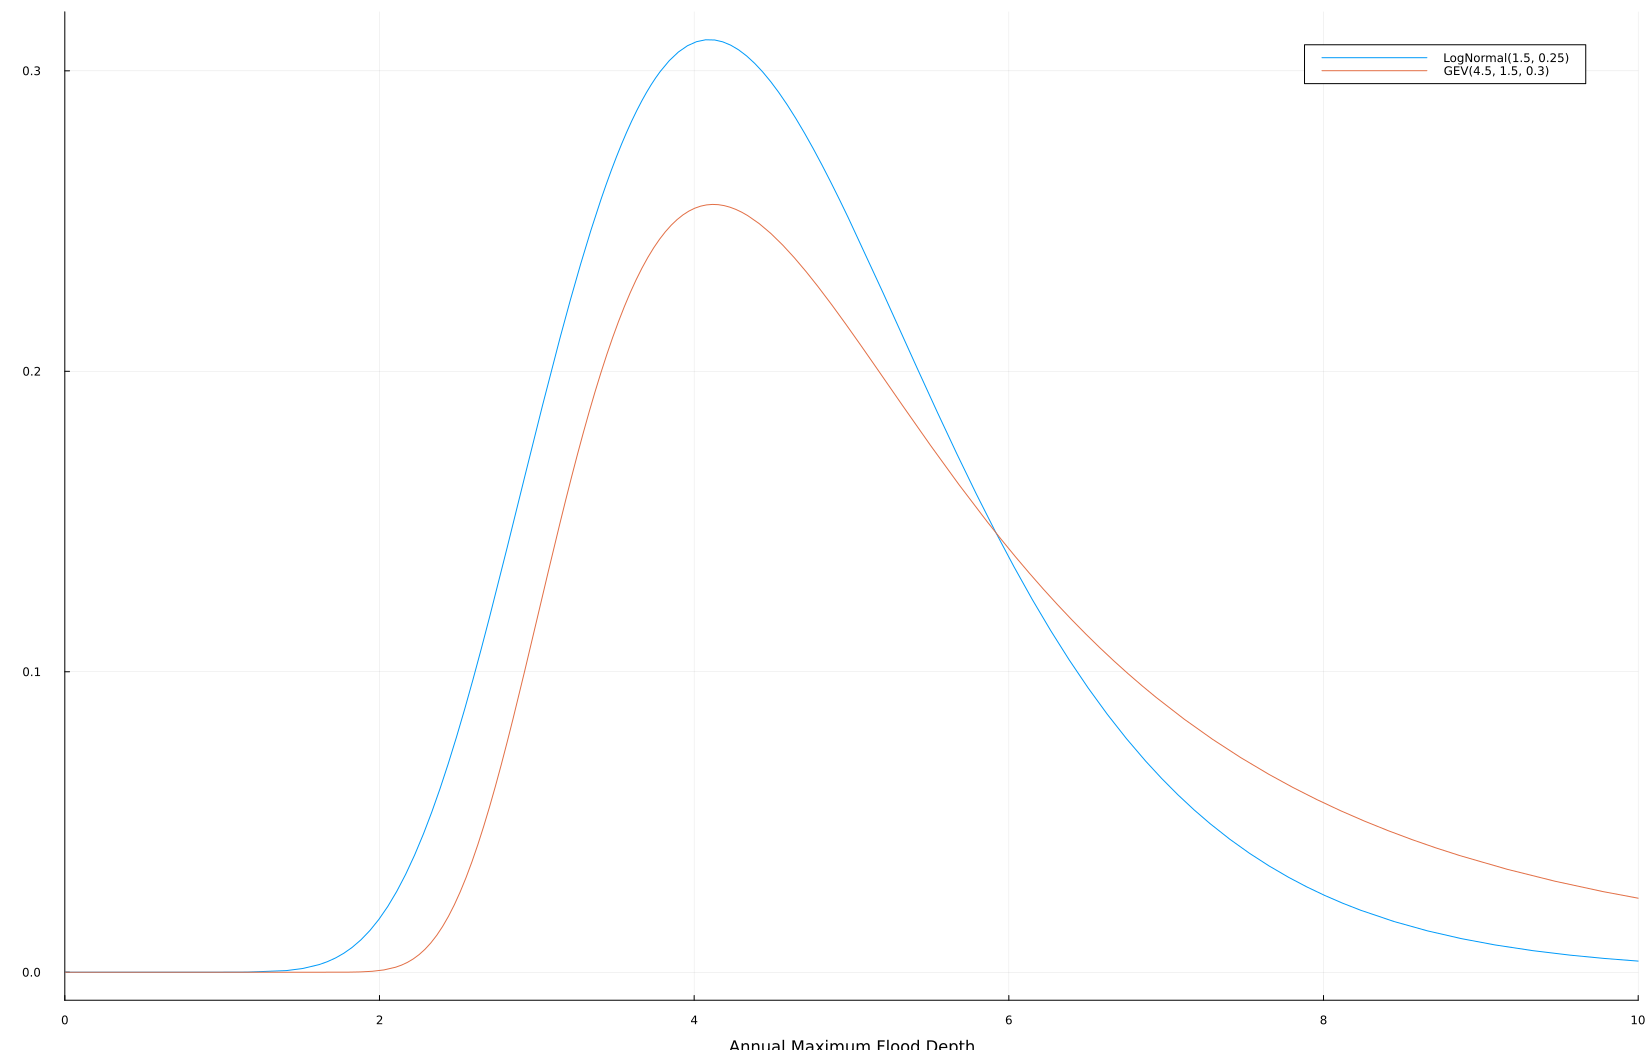
\includegraphics{ex07_files/mediabag/ex07_files/figure-pdf/fig-dists-output-1.pdf}

}

\caption{\label{fig-dists}Distributions used in this Monte Carlo
exercise.}

\end{figure}%

What are the Monte Carlo estimates of the expected value and the 99\%
quantile for the annual maximum damage the structure would suffer for
each of these flood hazard distributions? How did you ensure your sample
size was sufficiently large? Why do you think the estimates differed or
did not differ?

\subsection{References}\label{references}



\end{document}
